\chapter{Sustav kontinuiranog razvoja na primjeru Web programa}
Servis Github korišten je za reviziju koda te je projekt nazvan \textit{diplomski-go}. Također,
Jenkins je instaliran zajedno s osnovnim dodacima koji su potrebno za ovaj projekt. Nakon objave
prve verzije programa, izrađen je Jenkins posao koji izgrađuje Docker sliku te objavljuje na
službeni Docker repositorij. Takvu sliku će preuzeti servis za menadžment te pokreće Docker
kontejner. Nakon što je kontejner spreman, Nginx počinje preusmjerivati zahtjeve na njega.

\section{Aplikacija za izračun fibonaccijevog broja}
Za testiranje kontinuiranog razvoja izrađena je web programa za izračun fibonaccijevog broja u Go
programskom jeziku. Fibonaccijev broj definiran je rekurzijskom relacijom:

\begin{equation*}
    f(n) = \begin{cases}
               0               & n = 0\\
               1               & n = 1\\
               f(n-1) + f(n-2) & n > 1
           \end{cases}
\end{equation*}

U prvoj iteraciji programa koristi se naivno, rekurzivno rješenje vremenske i memorijske
kompleksnosti $O(2^N)$. Prilikom primitka HTTP zahtjeva, programa pokreće računanje fibonaccijevog
broja tako da zbroji rješenja prijašnje dvije iteracije fibonaccijevog broja. Na primjer, ako je
zatražen broj pet, funkcija vraća zbroj dvije fibonacci funkcije, jedna s parametrom četiri, a druge
s tri. Implementacija je prikazana kodom~\ref{03fibv1}.

\lstset{caption={Fibonacci v1}, label=03fibv1}
\begin{lstlisting}
func fibonacci(n uint64) uint64 {
	if n == 0 {
		return 0
	} else if n == 1 {
		return 1
	} else {
		return fibonacci(n-1) + fibonacci(n-2)
	}
}
\end{lstlisting}

Kako bi se provjerila ispravnost koda, napisani su jednostavni testovi jedinice, prikazano
kodom~\ref{03fibunit}.

\lstset{caption={Testiranje jedinice}, label=03fibunit}
\begin{lstlisting}
func TestFibonacci(t *testing.T) {
	assert.Equal(t, uint64(5), fibonacci(5))
	assert.Equal(t, uint64(8), fibonacci(6))
	assert.Equal(t, uint64(89), fibonacci(11))
}
\end{lstlisting}

U glavnoj funkciji koja se poziva prilikom pokretanje programa, \textit{main}, pokrenut je HTTP
servis koji je zadužen za posluživanje HTTP zahtjeva. Pokretanje HTTP servisa dan je
kodom~\ref{03fibhttp}.

\lstset{caption={HTTP servis}, label=03fibhttp}
\begin{lstlisting}
func fibonacciHandler(w http.ResponseWriter, r *http.Request) {
	n, err := strconv.ParseUint(r.URL.Query().Get("broj"), 10, 64)
	if err != nil {
		w.WriteHeader(http.StatusBadRequest)
		w.Write([]byte("Parametar broj mora biti prirodni broj."))
		return
	}
	w.WriteHeader(http.StatusOK)
	w.Write([]byte(strconv.FormatUint(fibonacci(n), 10)))
}

func healthHandler(w http.ResponseWriter, r *http.Request) {
	w.WriteHeader(http.StatusOK)
	w.Write([]byte("OK"))
}

func main() {
	http.HandleFunc("/", fibonacciHandler)
	http.HandleFunc("/health", healthHandler)

	log.Fatal(http.ListenAndServe(":8080", nil))
}
\end{lstlisting}

\section{Jenkins posao za izgradnju i objavu Docker slike}
Za Jenkins posao koji izrađuje Docker sliku i objavljuje u Docker repositorij odabrana je je Jenkins
linija. Jenkins linija je isprogramirana i spremljena u datoteci~\textit{Jenkinsfile} unutar
fibonacci projekta. Jenkins linija se sastoji od četiri faze: dohvaćanje koda preko Git projekta,
pokretanje testova jedinica, izgradnja Docker slike te objava Docker slike u javni Docker
repositorij. Na slici~\ref{fig:03jenkins_pipeline} prikazana je Jenkins linija.

\begin{figure}
    \centering
    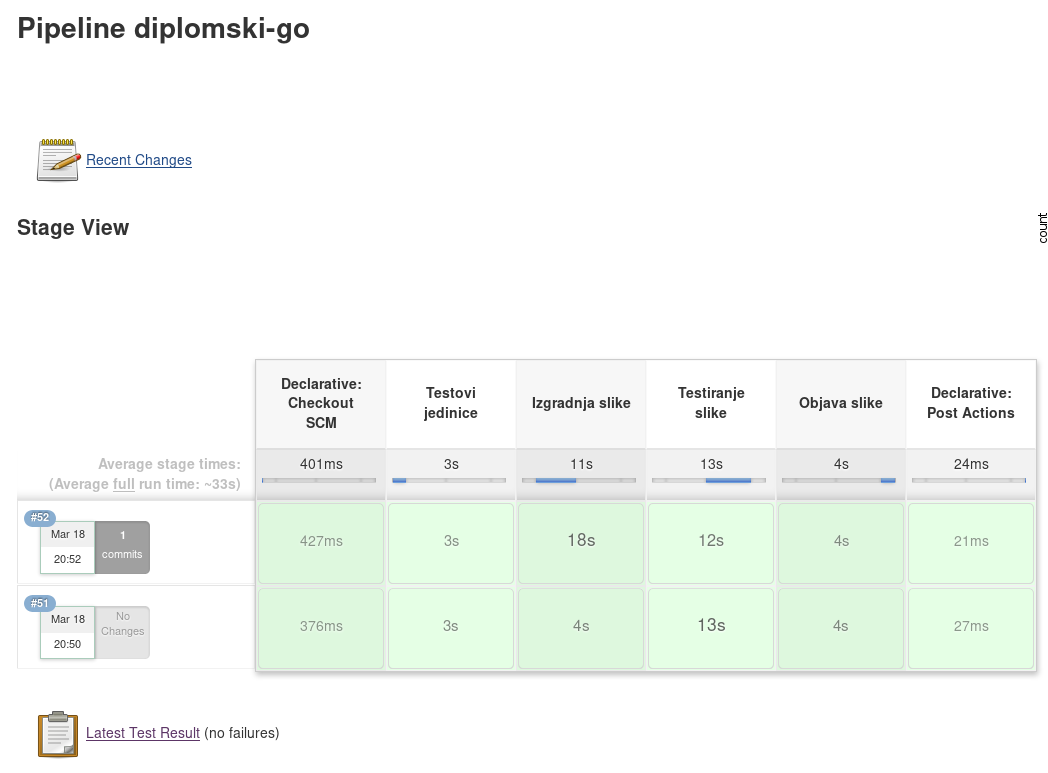
\includegraphics[width=0.8\textwidth]{img/03/jenkins_pipeline.png}
    \caption{Jenkins linija za izgradnju i objavu slike}%
    \label{fig:03jenkins_pipeline}
\end{figure}

Jenkins linija podešena je da periodički provjerava Git projekt, točnije svake minute. Ukoliko je
došlo do promjene u Git projektu, pokreće Jenkins liniju.

U prvoj fazi Jenkins kopira Git projekt koji se poslužuje preko Github servisa. Git projekt javno je
dostupan tako da nije potrebno podesiti autorizaciju. Nakon što je Git projekt kopiran, Jenkins
uspoređuje razliku između prijašnje i trenutnačne verzije te ih prikazuje korisniku.

U drugoj fazi pokreće se testovi jedinice unutar Docker kontejnera. Fibonacci aplikacija sastoji se
od jednog testa jedinice koji ispituje 3 ulaza. Ukoliko dođe do greške, Jenkins linija se prekida.
Pomoću ~\textit{junit} skripte, Jenkins objavljuje rezultate testova, kao i vrijeme izvođenja.

U trećoj fazi aplikacija se kompajlira i objavljuje sprema unutar Docker slike. Treća i druga faza
dijele istu baznu Docker sliku. Stoga, inženjer može biti siguran da su sve biblioteke dostupne
ukoliko su pokrivene testovima jedinice. Docker slika se označuje s trenutnom verzijom izgradnje
(engl.~\textit{build number}) te se objavljuje na Docker repositorij. Kako bi se slika mogla
objaviti, potrebno je podesiti Docker autorizaciju unutar Jenkins sustava.

U zadnjoj fazi, Docker slika se označuje sa specijalnom oznakom \textit{latest}. Ta oznaka označuje
da je Docker slika spremna za uporabu od strane klijenata.

\section{Servis za menadžment}
Nakon što je slika objavljena na Docker repositoriju, poslužitelj ju treba preuzeti i pokrenuti.
Taj algoritam pokreće se na servisa za menadžment, koji je također napisan u Go programskom jeziku.
Servis ima dva moguća stanja prilikom pokretanja: Docker kontenjer se već izvodi na poslužitelju te
prazno stanje. Ukoliko kontenjer postoji, potrebno je učitati informacije o portu. Nakon učitavanja,
servis počinje periodički provjeravati je li objavljanje nova verzija aplikacije.  Ukoliko postoji
nova verzija, servis mora preuzeti Docker sliku i pokrenuti Docker kontenjer na portu koji već nije
zauzet. Nakon pokretanja, periodički se provjerava ispravnost aplikacija pomoću provjere zdravlja
(engl.~\textit{health check}). Kada aplikacija bude zdrava, obaviještava se Nginx o novoj aplikaciji
te se preusmjerava promet. Dijagram toka prikazan je slikom~\ref{fig:03servismanagement}.

\begin{figure}[h]
    \centering
    \begin{tikzpicture}[
        scale=1.0,
        node distance=1cm,
        text width=3.5cm,
        text centered,
        block/.style={
            rectangle,
            draw,
            text width=10em,
            text centered,
            rounded corners,
        },
        process/.style={
            rectangle,
            draw,
            text width=10em,
            text centered,
        },
        decision/.style={
            diamond,
            draw,
            text width=4em,
            text badly centered,
            inner sep=0pt,
        },
        arrow/.style={
            thick,->,>=stealth
        },
    ]
        \node [block] (start) {POČETAK};
        \node [decision, below=of start] (exists) {Kontenjer postoji?};

        \node [right=of exists] (e1) {};
        \node [process, below=of e1] (readstate) {Učitaj kontenjere};

        \node [process, below=of exists] (checkversion) {Provjeri \textit{latest} verziju slike};

        \node [left=of checkversion] (e2) {};

        \node [decision, below=of checkversion] (newversion) {Nova verzija?};

        \node [process, below=of newversion] (launch) {Pokreni najnoviju verziju u kontejneru};
        \node [process, below=of launch] (save) {Spremni novu Nginx konfiguraciju};
        \node [process, below=of save] (shutdown) {Ugasi stari kontejner};

        \draw [arrow] (start) -- (exists);
        \draw [arrow] (exists) -| node[anchor=south east] {DA} (readstate);
        \draw [arrow] (readstate) |- (checkversion);
        \draw [arrow] (exists) -- node[xshift=-5mm] {NE} (checkversion);
        \draw [arrow] (checkversion) -- (newversion);
        \draw [arrow] (newversion) -- node[anchor=south] {NE} ++(-3cm,0cm) |- (checkversion);

        \draw [arrow] (newversion) -- node[xshift=-5mm] {DA} (launch);
        \draw [arrow] (launch) -- (save);
        \draw [arrow] (save) -- (shutdown);
        \draw [arrow] (shutdown) -- ++(+4.5cm,0cm) |- (checkversion);
    \end{tikzpicture}
    \caption{Dijagram toka servisa za menadžment}%
    \label{fig:03servismanagement}
\end{figure}


